\documentclass[10pt]{article}
\usepackage{times}
\usepackage{multicol}   
\usepackage{graphicx}   
\usepackage{amsmath}    
\usepackage{hyperref}   
\usepackage{float}      
\usepackage{geometry}   
\usepackage{booktabs}   % For better tables
\usepackage[export]{adjustbox}
\geometry{margin=1in}

\usepackage[backend=bibtex,style=numeric]{biblatex}
\addbibresource{references.bib}

\title{Quantum Weirdness: Exploring Quantum Error Correction}
\author{Andry Lloyd Paez \\
San Jose State University}
\date{}

\begin{document}

\maketitle

\begin{abstract}
Quantum computers are highly susceptible to noise, which can lead to errors that jeopardize computations. Quantum Error Correction (QEC) offers a robust way to protect quantum information from such errors. This project focuses on demonstrating the efficiency of the Shor Code, one of the foundational quantum error-correcting codes. By simulating noisy quantum systems with and without error correction, we highlight the effectiveness of QEC; however, in order to accurately test it's effectiveness, we need a real environment. To accomplish this, we apply QEC to real quantum hardware, measure the results, and discuss the challenges accompanied by using real quantum hardware.
\end{abstract}

% Begin two-column layout
\begin{multicols}{2}

    \section*{Introduction}
    Quantum computing is a revolutionary model that uses the principles of quantum mechanics to perform computations beyond the reach of classical computers. Central to its power are the phenomena of superposition and entanglement, which enable quantum bits, or qubits, to exist in multiple states simultaneously and share correlations across distances. However, these advantages are accompanied by significant challenges, particularly the issue of noise. Quantum systems are inherently fragile, and errors such as bit-flips and phase-flips can easily disrupt computations, reducing their reliability.\cite{bernhardt}
    
    Motivated by these challenges, this project seeks to explore how quantum error correction (QEC) can address the problem of noise in quantum systems. Specifically, we focus on visualizing and implementing the Shor Code, a foundational QEC scheme that protects quantum information by redundantly encoding logical qubits into multiple physical qubits (ancillary qubits). By simulating noisy environments and testing on real quantum hardware, we aim to demonstrate the effectiveness of error correction techniques in mitigating these errors.
    
    \subsection*{Theory}
    To understand quantum error correction, it is essential to grasp the basics of quantum computing. A qubit, the fundamental unit of quantum information, can exist in a superposition state described by the equation:
    \[
    |\psi\rangle = \alpha|0\rangle + \beta|1\rangle
    \]
    where \( |\alpha|^2 \) and \( |\beta|^2 \) represent the probabilities of measuring the qubit in the \( |0\rangle \) or \( |1\rangle \) state, respectively. The normalization condition \( |\alpha|^2 + |\beta|^2 = 1 \) ensures that these are proper probabilities.
    
    Quantum computations are visualized using quantum circuits, where qubits are represented as horizontal lines and operations are depicted as gates. These circuits provide a framework for manipulating qubits to perform specific tasks.\cite{bernhardt}
    \begin{figure}[H]
        \centering
        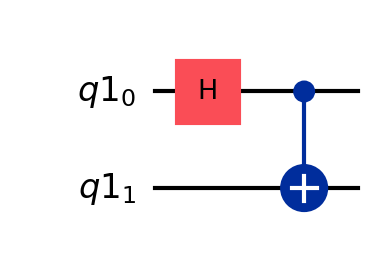
\includegraphics[width=0.8\columnwidth]{figures/qc.png}
        \caption{A simple quantum circuit demonstrating superposition.}
        \label{fig:bell_circuit}
    \end{figure}
    
    Errors in quantum systems come in various forms. Bit-flip errors occur when a qubit transitions from \( |0\rangle \) to \( |1\rangle \) or vice versa, while phase-flip errors alter the relative phase between these states. These errors highlight the need for correction methods.
    
    The 3-bit repetition code provides a straightforward approach to error correction by encoding a single logical qubit into three physical qubits. This method protects against single bit-flip errors by relying on majority voting to determine the original state. Although effective for certain scenarios, it cannot handle more complex errors, such as phase flips.
    
    To address these limitations, the Shor Code extends the concept of redundancy by encoding one logical qubit into nine physical qubits. This scheme combines the principles of bit-flip and phase-flip protection, providing a comprehensive error-correction mechanism.\cite{roffe} The Shor Code is visualized in Figure \ref{fig:shor_circuit}.
    \begin{figure}[H]
        \centering
        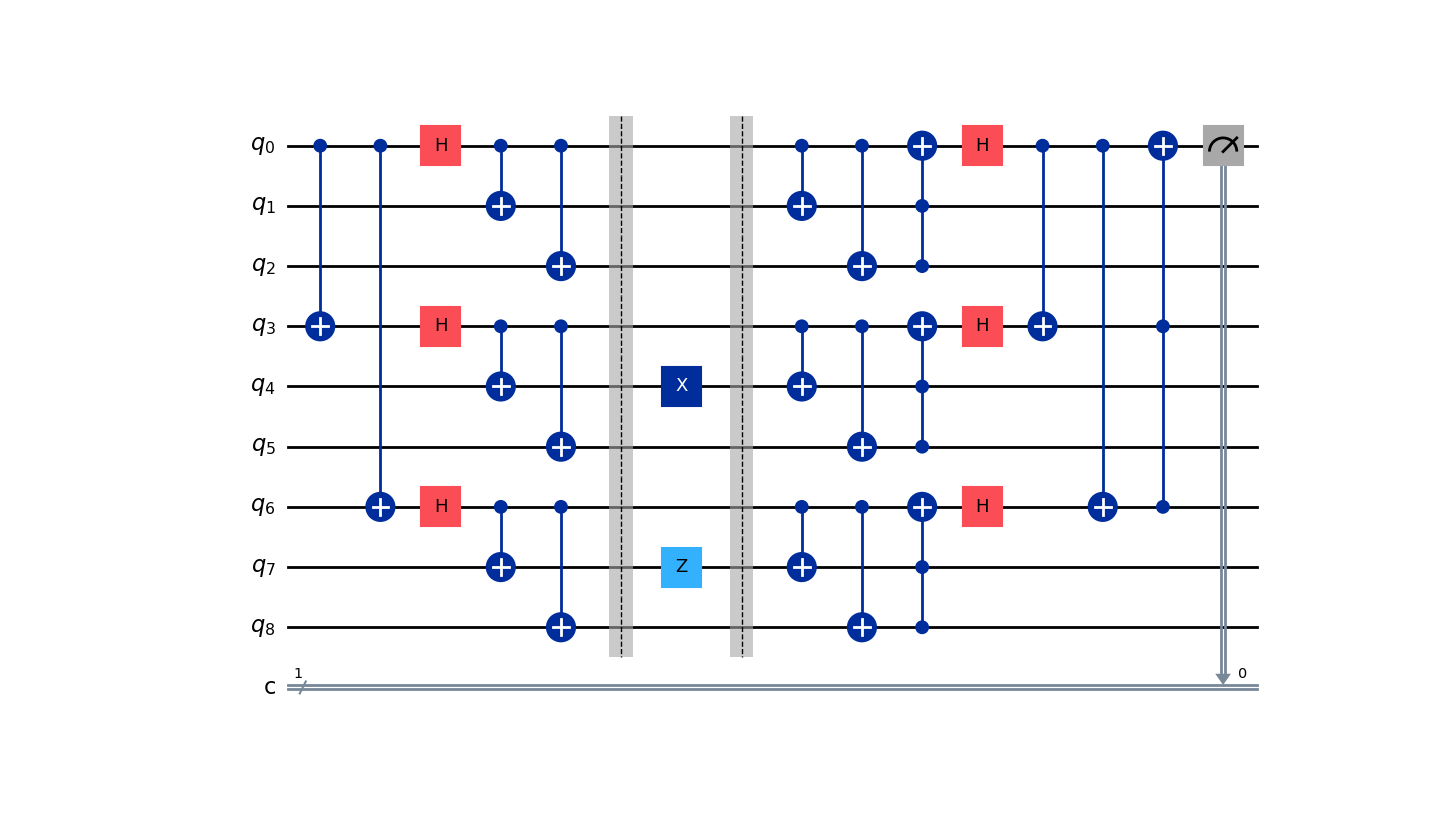
\includegraphics[width=1.0\columnwidth]{figures/shor.png}
        \caption{The Shor Code Circuit used for error correction.}
        \label{fig:shor_circuit}
    \end{figure}
    
    Through this project, we aim to investigate how these codes perform in both simulated and real hardware environments, offering insights into the current capabilities and limitations of quantum error correction.

\section*{Methods}
The methodology for this project involved both simulated environments and real quantum hardware to study and compare the effectiveness of quantum error correction. Initially, we constructed a noisy simulation environment using QiskitAer to model quantum errors such as bit-flips and phase-flips. This approach allowed for controlled testing of error-correcting codes in a highly customizable setup.

The implementation was divided into modular functions. Separate encoding and decoding functions were created for both the 3-bit repetition code and Shor's Code. These functions systematically applied gates to propagate the logical qubit's state to ancillary qubits, introducing redundancy to correct errors. A noise model was then incorporated to simulate errors between encoding and decoding stages.

For testing on real quantum hardware, IBM Channels were accessed via the Qiskit Runtime. The "least\_busy" function was used to identify an appropriate backend, and circuits were transpiled to match the device-specific quantum instruction set architecture (ISA). Key results, such as measurement counts, were collected and analyzed to evaluate the fidelity of error correction.\cite{qiskit}

By combining simulations and real hardware trials, this methodology provided a comprehensive comparison of theoretical expectations and practical outcomes for quantum error correction.

\section*{Results and Discussion}
\subsection*{3-Bit Repetition Code Results}
\begin{figure}[H]
    \centering
    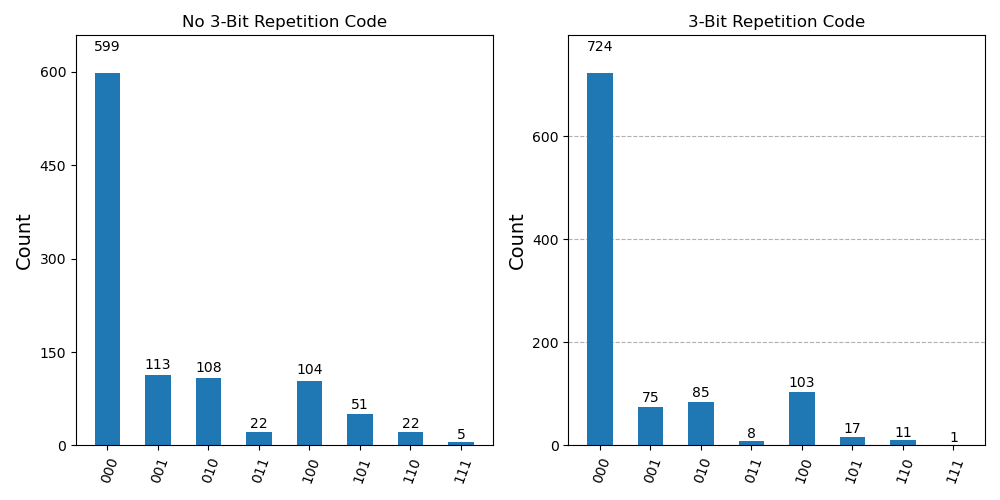
\includegraphics[width=1.0\columnwidth]{figures/3-bit_results.png}
    \caption{Measurement results for the 3-Bit Repetition Code (right) vs. No Error Correction (left).}
    \label{fig:3_bit_results}
\end{figure}

Figure \ref{fig:3_bit_results} presents the measurement results comparing the 3-Bit Repetition Code to a circuit with no error correction. Without error correction, the fidelity was calculated as 0.902, corresponding to an error rate of 9.77\%. In contrast, the implementation of the 3-Bit Repetition Code improved fidelity to 0.964, reducing the error rate to 3.61\%. These results demonstrate the effectiveness of the 3-Bit Repetition Code in mitigating errors, though its ability to handle only single bit-flip errors highlights its limitations compared to more advanced error correction codes.

\subsection*{Shor Code Simulation}
\begin{figure}[H]
    \centering
    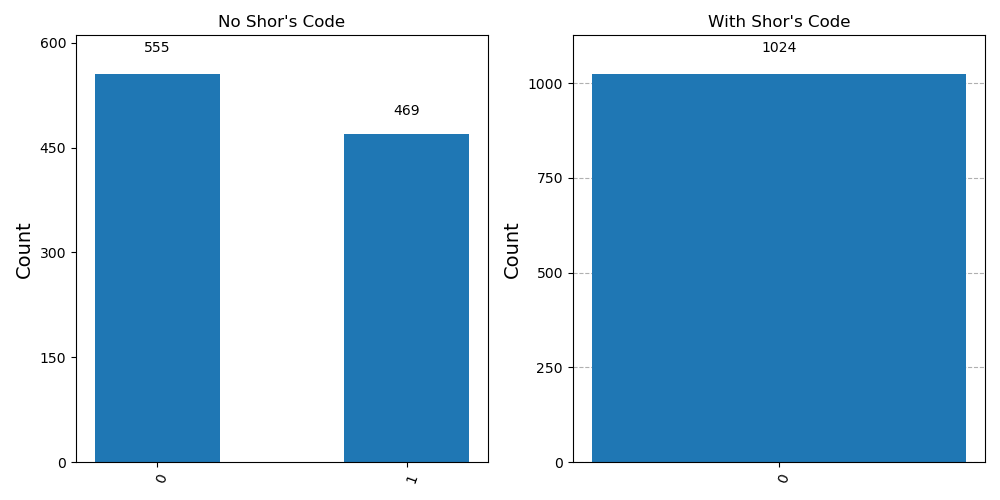
\includegraphics[width=1.0\columnwidth]{figures/shors_result_sim.png}
    \caption{Simulated results: Shor's Code (right) vs. No Error Correction (left).}
    \label{fig:shor_sim}
\end{figure}
The simulated results for the Shor Code clearly demonstrated the code's theoretical effectiveness in correcting errors in quantum systems. Figure \ref{fig:shor_sim} compares measurement outcomes with and without the Shor Code applied. Without error correction, the fidelity was 0.542, corresponding to an error rate of 45.80\%. In contrast, with the Shor Code applied, the simulated fidelity improved dramatically to 1.000, eliminating errors entirely under the tested conditions.

The significant disparity in results highlights the theoretical value of quantum error correction when implemented correctly. These findings underscore the importance of redundancy in encoding quantum information, as introduced by the Shor Code.

\subsection*{Shor Code on Real Hardware}
\begin{figure}[H]
    \centering
    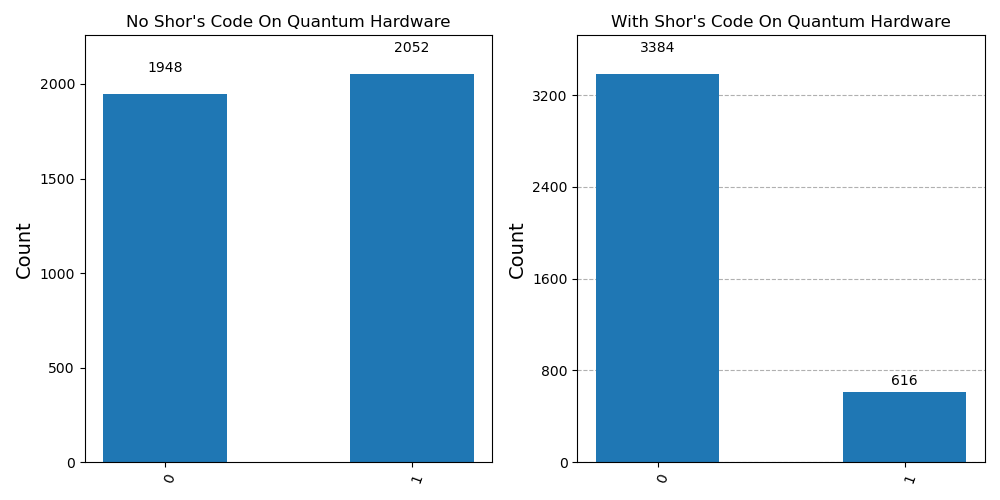
\includegraphics[width=1.0\columnwidth]{figures/shors_results.png}
    \caption{Real hardware results: Shor's Code (right) vs. No Error Correction (left).}
    \label{fig:shor_real}
\end{figure}

When implemented on real quantum hardware, the results for the Shor Code showed noticeable improvement in fidelity compared to circuits without error correction, although the performance was not as ideal as in simulations. Figure \ref{fig:shor_real} presents the measurement results. Without error correction, the fidelity was calculated to be 0.487, corresponding to an error rate of 51.30\%. With the Shor Code applied, the fidelity improved to 0.846, reducing the error rate to 15.40\%.

These results emphasize the challenges of deploying quantum error correction on real hardware, where additional noise sources, such as gate errors and decoherence, limit the overall effectiveness of the correction scheme. Despite these limitations, the Shor Code demonstrated its ability to mitigate errors to a significant extent, showcasing its potential for fault-tolerant quantum computing in the future.

\section*{Conclusion}
This project demonstrates the critical role of quantum error correction (QEC) in mitigating noise and improving the reliability of quantum computations. The 3-bit repetition code provided a foundational understanding of redundancy-based error correction, effectively addressing single bit-flip errors but limited in handling more complex noise scenarios.

Building upon these principles, the Shor Code demonstrated its potential to correct both bit-flip and phase-flip errors, achieving significant accuracy improvements in both simulated environments and real quantum hardware. While simulations showed ideal results, the performance on real hardware revealed the limitations imposed by noise, gate fidelity, and current technological constraints. Nevertheless, the Shor Code consistently outperformed circuits without error correction, highlighting its importance as a cornerstone of fault-tolerant quantum computing.

The results of this study emphasize the necessity of advanced QEC techniques for bridging the gap between theoretical capabilities and practical quantum computing. As hardware reliability improves, error-correcting codes like the Shor Code will become essential for unlocking the full potential of quantum computation.


\section*{Acknowledgments}
Thanks to the instructors, peers, and online resources that supported this project.

\end{multicols}

% References
\printbibliography
\end{document}
